\documentclass[a4paper]{extarticle}
\usepackage[utf8]{inputenc}
\usepackage[a4paper, margin=1in]{geometry}

\usepackage{amssymb}
\usepackage{amsmath}
\usepackage{enumitem}
\usepackage{tcolorbox}
\usepackage{fancyhdr}
\usepackage{graphicx}
\usepackage{float}

\setlength{\parindent}{0em}
\setlength{\parskip}{0.4em}

\definecolor{theoremblue}{RGB}{1, 73, 124}
\definecolor{corollaryblue}{RGB}{70, 143, 175}
\definecolor{exampleblue}{RGB}{137, 194, 217}

\newtcolorbox{tbox}{colback=theoremblue!20,colframe=theoremblue,
boxrule=0pt,arc=0pt,boxsep=2pt,left=2pt,right=2pt,leftrule=2pt}

\newtcolorbox{cbox}{colback=corollaryblue!20,colframe=corollaryblue,
boxrule=0pt,arc=0pt,boxsep=2pt,left=2pt,right=2pt,leftrule=2pt}

\newtcolorbox{ebox}{colback=exampleblue!20,colframe=exampleblue,
boxrule=0pt,arc=0pt,boxsep=2pt,left=2pt,right=2pt,leftrule=2pt}

\title{EnpRisk - Lecture Notes Week 5}
\author{Ruben Schenk, ruben.schenk@inf.ethz.ch}
\date{\today}

\pagestyle{fancy}
\fancyhf{}
\rhead{ruben.schenk@inf.ethz.ch}
\rfoot{Page \thepage}
\lhead{EnpRisk - Lecture Notes Week 5}

\begin{document}

\maketitle
\newpage

\subsection{Wrapping up The Deal}

Before we draft the legal documents, we need to agree on the most important principles of the deal:

\begin{itemize}
    \item The amount invested, and how it will be made available
    \item The value of the company
    \item The cap table, who owns what percentage of the company
    \item The governance principles
\end{itemize}

\subsubsection{The Amount Invested}

The previous part on corporate finance and company valuation, we explained how to calculate cash flows and cash position. Based on all the information gathered during the due diligence, the investor will calculate a number of cash burn scenarios. This will be used to assess the amount of capital that needs to be invested.

\textit{Capital invested in a startup is used for burning cash, so, it is important to have a good understanding of different cash burn scenarios!}

In the example below, we decided to invest 2M Euro's, which was our base case scenario. The investment amount turned out to be too small and follow-up rounds were needed:

\begin{figure}[H]
    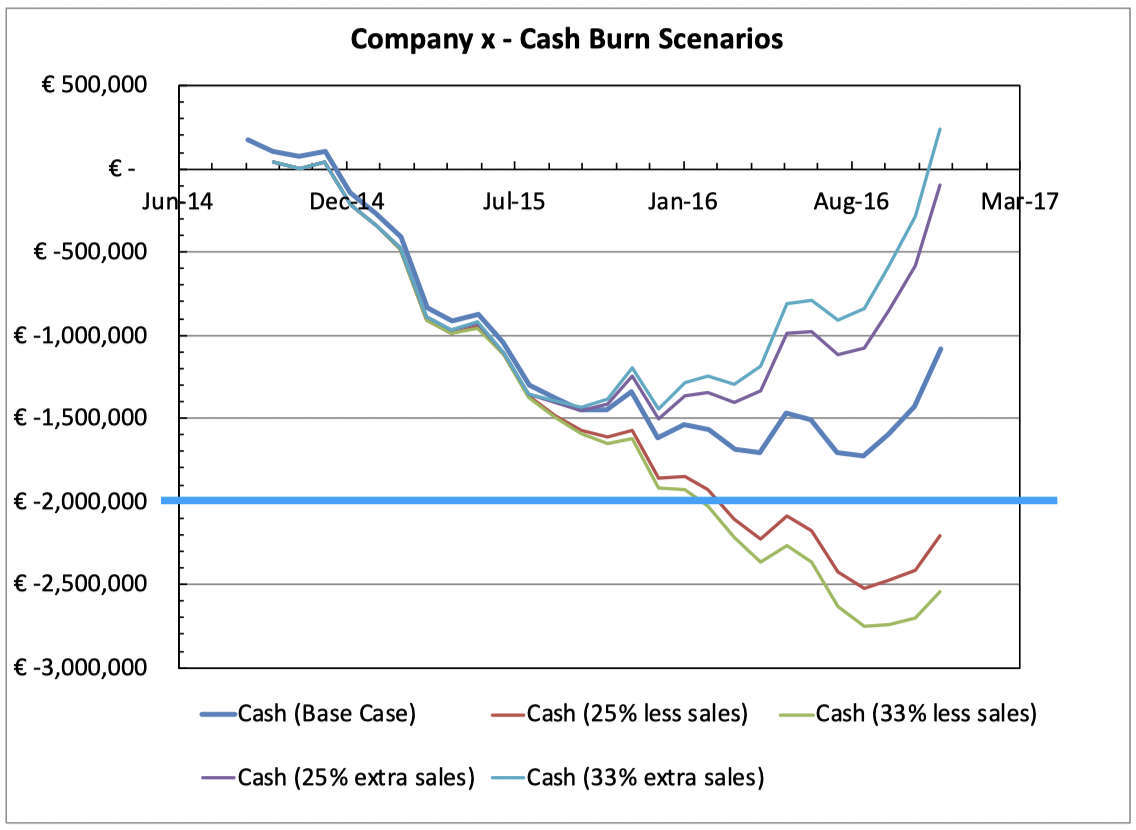
\includegraphics[width=9cm]{../images/EnpRisk_Fig5-1}
    \centering
\end{figure}

As a founder, it is important to negotiate for a strong \textbf{cash buffer.} If the cash burn is higher than expected, you may need to find new capital in a situation under stress. At that time your company valuation will be low, and you will dilute (i.e. start losing ownership of the company).

\subsubsection{The Value of The Company}

Some common metrics, which we already defined previously, are:

\begin{itemize}
    \item \(\Delta WC\) = Change in accounts receivable + change in inventory - change in accounts payable
    \item Accounts receivable = Sum of all invoices send out to customers that have not been paid yet
    \item Accounts payable = Sum of all invoices received from vendors that you have not paid yet
    \item Taxes: You only pay taxes when the cumulative EBT (Earnings before taxes) of the previous years is positive
    \item Depreciation: Not a cash flow item, it is a loss, but it's not a cash-out. The cash-out occurred at the time if the investment, so to got from P\&L to cash flow you have to add the non-cash items again.
\end{itemize}

\subsubsection{Cap Table}

With the value of the company determined, we can create the \textbf{pre- and post-money valuation and cap table:}

\begin{table}[H]
    \centering
    \begin{tabular}{|l|l|l|}
    \hline
    \textbf{Pre-money} & \textbf{Ownership} & \textbf{Value}  \\ \hline
    Founder 1          & $33.3\%$           & EUR $1'333'333$ \\ \hline
    Founder 2          & $33.3\%$           & EUR $1'333'333$ \\ \hline
    University         & $33.3\%$           & EUR $1'333'333$ \\ \hline
    \textbf{Total}     &                    & EUR $4'000'000$ \\ \hline
    \end{tabular}
    \caption{Pre-money cap table.}
    \label{tab:cap-table-01-pre-money}
 \end{table}

 \begin{table}[H]
    \centering
    \begin{tabular}{|l|l|l|}
    \hline
    \textbf{Post-money} & \textbf{Ownership} & \textbf{Value}  \\ \hline
    Investor           & $33.3\%$           & EUR $2'000'000$ \\ \hline
    Founder 1          & $22.2\%$           & EUR $1'333'333$ \\ \hline
    Founder 2          & $22.2\%$           & EUR $1'333'333$ \\ \hline
    University         & $22.2\%$           & EUR $1'333'333$ \\ \hline
    \textbf{Total}     &                    & EUR $6'000'000$ \\ \hline
    \end{tabular}
    \caption{Post-money cap table.}
    \label{tab:cap-table-01-post-money}
\end{table}

With this new investment, the initial owners get diluted by \(\frac{1}{3}\), that is the pre-money valuation of \(4M\), divided by the post-money valuation of \(6M\). In other words, \(\frac{1}{3}\) ownership becomes \(\frac{2}{9}\).

\subsubsection{Governance Principles}

The \textbf{governance principles} are outlining the responsibility, the composition, and the authority (the decision-making process) of the management team (MT), the supervisory board (SVB), and the general meeting of shareholders (GMS) of the company.

This allows for an efficient management of the company based on objective criteria and processes independently of existing persons and historical relationships.

\subsection{Corporate Bodies}

The \textbf{corporate bodies} of a company are usually made out of the following three groups: General meeting of shareholders, supervisory board, and management team.

The \textit{management team} is to do day-to-day affairs. Furthermore:

\begin{itemize}
    \item Has the authority to decide in line with the annual budget and business plan
    \item In case of significant deviation from the budget and business plan, the decision is escalated to the board
\end{itemize}

The \textit{supervisory board} is to do supervision. In particular:

\begin{itemize}
    \item Composed of representatives of the shareholders, independent board members, and senior management
    \item Composition and voting rights are clearly defined in the shareholders' agreement
    \item Must supervise and advise the management and oversee the general affairs within the company
    \item Should be guided by the interests of the company
\end{itemize}

Finally, the \textit{general meeting of shareholders} is responsible for value creation. More specifically:

\begin{itemize}
    \item Composed of the shareholders of the company
    \item Meets at least once per year to approve the annual accounts, discharge the board and follow up and/or adapt the value creation plan
    \item Appoints the members of the supervisory board and sometimes also members of the management team
\end{itemize}

\subsection{Legal Documents}

Once the amount invested, the value of the company, the cap table, and the governance principles are agreed upon, the legal documents are drafted.

The main documents are the following:

\begin{itemize}
    \item Subscription Agreement (the transaction)
    \item Shareholders Agreement (governance and organization)
    \item Management Agreement (day-to-day operations)
\end{itemize}

\subsubsection{Subscription Agreement}

A \textbf{subscription agreement} is between a company and a private investor to sell a specific number of shares at a specific price. It contains, amongst others, information regarding the amount invested, the cap table, issue of new shares or transfer of existing shares, payment conditions, etc.

Some agreements include a specific rate of return that investors are guaranteed to receive (the so-called \textit{preference shares.})

\subsubsection{Shareholders Agreement}

A \textbf{shareholder's agreement} describes how the company should be operated and outlines shareholder's rights and obligations. It is intended to make sure that all shareholders are treated fairly and that their rights are protected.

It also outlines the governance principles: the responsibility, the composition and the authority of the management team, the supervisory board, and the general meeting of shareholders of the company.

Furthermore, it describes the exit scenarios (i.e. the transfer of shares) with specific care for the rights of minority as well as majority shareholders.

The different EXIT strategies are as follows:

\begin{itemize}
    \item \textit{Lock-up:} A predetermined amount of time when shareholders are restricted from selling their shares.
    \item \textit{Right of first refusal:} After the lock-up period, when one shareholder can sell shares to a third party, other shareholders must be given the opportunity to match the price and buy shares instead of the third party.
    \item \textit{Drag along} (protection of majority): A drag along right allows a majority shareholder of a company to force the remaining minority shareholders to accept an offer from a third part to purchase the whole company at the same price, terms and conditions.
    \item \textit{Tag along} (protection of minority): Tag along rights are the inverse of drag along rights. When a majority shareholder sells their shares, a tag along right will entitle the minority shareholder to participate in the sale at the same time for the same price, terms and conditions.
\end{itemize}

\subsubsection{Management Agreement}

Finally, the \textbf{management agreement} is an agreement between the management and the company outlining:

\begin{itemize}
    \item Expected management services
    \item Management fees
    \item Targets and objectives
    \item Intellectual property rights
    \item etc.
\end{itemize}

\end{document}